\documentclass[12pt, twoside]{article}
\usepackage[letterpaper, margin=1in, headsep=0.2in]{geometry}
\setlength{\headheight}{0.6in}
%\usepackage[english]{babel}
\usepackage[utf8]{inputenc}
\usepackage{microtype}
\usepackage{amsmath}
\usepackage{amssymb}
%\usepackage{amsfonts}
\usepackage{siunitx} %units in math. eg 20\milli\meter
\usepackage{yhmath} % for arcs, overparenth command
\usepackage{tikz} %graphics
\usetikzlibrary{quotes, angles}
\usepackage{graphicx} %consider setting \graphicspath{{images/}}
\usepackage{parskip} %no paragraph indent
\usepackage{enumitem}
\usepackage{multicol}
\usepackage{venndiagram}

\usepackage{fancyhdr}
\pagestyle{fancy}
\fancyhf{}
\renewcommand{\headrulewidth}{0pt} % disable the underline of the header
\raggedbottom
\hfuzz=2mm %suppresses overfull box warnings

\usepackage{hyperref}

\fancyhead[LE]{\thepage}
\fancyhead[RO]{\thepage \\ Name: \hspace{4cm} \,\\}
\fancyhead[LO]{BECA / Dr. Huson / Geometry\\*  Unit 11: Circle angles, sectors, arcs \\* 27 February 2023}

\begin{document}

\subsubsection*{11.1 Extension: Radian measure}
\begin{enumerate}
\item A \emph{unit} circle with a radius $r=1$ is divided in quarters. One sector, $AOB$, is shaded as shown.
  \begin{multicols}{2}
  \raggedcolumns
  \begin{enumerate}[itemsep=1.5cm]
    \item Find the circumference in terms of $\pi$. ($C=2\pi r$)
    \item Write down $m \angle AOB$ in \emph{degrees}.
    \item Find the \emph{length} of the arc $\wideparen{AB}$ in terms of $\pi$.
  \end{enumerate}
  \begin{tikzpicture}[scale=0.8]
    \fill [lightgray]
    (0,0)--(0:4) arc (0:90:4)--(0,0);
    \draw (0,0) circle[radius=4];
    \draw [thick, <->] (0:0.75) arc (0:90:0.75);
    \draw [thick, <->] (0:4) arc (0:90:4);
    \draw [thick]
    (0:4) node[right] {$A$}--
    (0,0) node[below left] {$O$}--
    (90:4) node[above] {$B$};
    \draw [thick, dotted](0:-4)--(0,0)--(-90:4);
    \fill (0,0) circle[radius=.1];
    \node at (45:4.5) {$?$};
    \node at (-10:2) {$1$};
  \end{tikzpicture}
  \end{multicols}

\item The length of the arc of a unit circle is a measure of the central angle called \emph{radians}. The circumference of the full circle is $2 \pi = 360^\circ$.\\[0.25cm]
Mark each angle with its radian measure.
  \begin{multicols}{2}
  \raggedcolumns
  \begin{enumerate}
    \item One half of a circle $180^\circ$\\
    \begin{tikzpicture}[scale=0.6]
      \fill [lightgray]
      (0,0)--(0:4) arc (0:180:4)--(0,0);
      \draw (0,0) circle[radius=4];
      \draw [thick, <->] (0:0.75) arc (0:180:0.75);
      \draw [thick, <->] (0:4) arc (0:180:4);
      \draw [thick]
      (0:4)--(0,0) node[below left] {$O$}--(180:4);
      %\draw [thick, dotted](0:-4)--(0,0)--(120:4);
      \fill (0,0) circle[radius=.1];
      \node at (90:1.5) {$180^\circ$};
      \node at (-10:2) {$1$};
    \end{tikzpicture}
    \item One sixth of the circle $60^\circ$\\
    \begin{tikzpicture}[scale=0.6]
      \fill [lightgray]
      (0,0)--(0:4) arc (0:60:4)--(0,0);
      \draw (0,0) circle[radius=4];
      \draw [thick, <->] (0:0.75) arc (0:60:0.75);
      \draw [thick, <->] (0:4) arc (0:60:4);
      \draw [thick]
      (0:4)--(0,0) node[below left] {$O$}--(60:4);
      \draw [thick, dotted](0:-4)--(0,0)--(120:4);
      \fill (0,0) circle[radius=.1];
      \node at (30:1.5) {$60^\circ$};
      \node at (-10:2) {$1$};
    \end{tikzpicture}
    \item One eighth of the circle $45^\circ$\\
    \begin{tikzpicture}[scale=0.6]
      \fill [lightgray]
      (0,0)--(0:4) arc (0:45:4)--(0,0);
      \draw (0,0) circle[radius=4];
      \draw [thick, <->] (0:0.75) arc (0:45:0.75);
      \draw [thick, <->] (0:4) arc (0:45:4);
      \draw [thick]
      (0:4)--(0,0) node[below left] {$O$}--(45:4);
      \draw [thick, dotted](0:-4)--(0,0)--(90:4);
      \fill (0,0) circle[radius=.1];
      \node at (20:1.5) {$45^\circ$};
      \node at (-10:2) {$1$};
    \end{tikzpicture}
    \item One third of a circle $120^\circ$\\
    \begin{tikzpicture}[scale=0.6]
      \fill [lightgray]
      (0,0)--(0:4) arc (0:120:4)--(0,0);
      \draw (0,0) circle[radius=4];
      \draw [thick, <->] (0:0.75) arc (0:120:0.75);
      \draw [thick, <->] (0:4) arc (0:120:4);
      \draw [thick]
      (0:4)--(0,0) node[left] {$O$}--(120:4);
      \draw [thick, dotted](240:4)--(0,0);
      \fill (0,0) circle[radius=.1];
      \node at (60:1.5) {$120^\circ$};
      \node at (-10:2) {$1$};
    \end{tikzpicture}
  \end{enumerate}
  \end{multicols}

\item Algebra view of \emph{radians} to \emph{degrees} using the formula $2 \pi = 360^\circ$ or $\pi = 180^\circ$.\\[0.25cm]
Apply the appropriate formula.
\begin{multicols}{2}
$\displaystyle r = d \times \frac{\pi}{180}$\\
$\displaystyle d = r \times \frac{180}{\pi}$
\end{multicols}
  \begin{multicols}{2}
  \raggedcolumns
  \begin{enumerate}
    \item $60^\circ = \hspace{0.15cm} ?$ radians\\[0.5cm]
    \begin{tikzpicture}[scale=1]
      \draw [thick, <->] (0:0.75) arc (0:60:0.75);
      \draw [thick, <->] (0:4) arc (0:60:4);
      \draw [dashed](0,0)--(4,0);
      \draw [thick]
      (0,0) node[below left] {$A$}--(60:4)--(2,0)--cycle;
      \fill (0,0) circle[radius=.1];
      \node at (30:1.5) {$60^\circ$};
    \end{tikzpicture}
    \item $30^\circ = \hspace{0.15cm} ?$ radians\\[0.5cm]
    \begin{tikzpicture}[scale=1]
      \draw [thick, <->] (0:0.75) arc (0:30:0.75);
      \draw [thick, <->] (0:4) arc (0:30:4);
      \draw [dashed](0,0)--(4,0);
      \draw [thick]
      (0,0) node[below left] {$A$}--(30:4)--(3.46,0)--cycle;
      \fill (0,0) circle[radius=.1];
      \node at (15:1.5) {$30^\circ$};
    \end{tikzpicture}
    \item $\displaystyle \frac{\pi}{4}  = \hspace{0.15cm} ?$ degrees\\[0.5cm]
    \begin{tikzpicture}[scale=1]
      \draw [thick, <->] (0:0.75) arc (0:45:0.75);
      \draw [thick, <->] (0:4) arc (0:45:4);
      \draw [dashed](0,0)--(4,0);
      \draw [thick]
      (0,0) node[below left] {$A$}--(45:4)--(2.82,0)--cycle;
      \fill (0,0) circle[radius=.1];
      \node at (22:1.5) {$?^\circ$};
      \node at (22:4.5) {$\displaystyle \frac{\pi}{4}$};
    \end{tikzpicture}
    \item $\displaystyle \frac{\pi}{8}  = \hspace{0.15cm} ?$ degrees\\[0.75cm]
    \begin{tikzpicture}[scale=1]
      \draw [thick, <->] (0:1) arc (0:22.5:1);
      \draw [thick, <->] (0:4) arc (0:22.5:4);
      \draw [dashed](0,0)--(4,0);
      \draw [thick]
      (0,0) node[below left] {$A$}--(22.5:4)--(3.7,0)--cycle;
      \fill (0,0) circle[radius=.1];
      \node at (12:1.8) {$?^\circ$};
      \node at (12:4.5) {$\displaystyle \frac{\pi}{8}$};
    \end{tikzpicture}
  \end{enumerate}
  \end{multicols}


\newpage
\item Do Now: Convert each set of units. One inch $= \displaystyle \frac{1}{12}$ foot or one foot $= 12$ inches.
  \begin{enumerate}[itemsep=1.5cm]
    \item How many feet are 30 inches?
    \item How many inches are 8.25 feet?
  \end{enumerate}

Example Greek letters are 
{\Large$\pi$, $\theta$, $\alpha$, $\Delta$, $\beta$, $\sigma$, $\Sigma$, $\epsilon$ \par}

\item Practice: Convert between units. \\[0.25cm]
General method: if $A = B$ multiply by $\displaystyle \frac{A}{B} \text{ or } \frac{B}{A}$. For example, $\pi \text{ radians}= 180 \text{ degrees}$ so \\
$\displaystyle r = d \times \frac{\pi}{180}$ and 
$\displaystyle d = r \times \frac{180}{\pi}$
\vspace{0.5cm}
  \begin{multicols}{2}
  \raggedcolumns
  \begin{enumerate}[itemsep=1.5cm]
    \item $40^\circ = \hspace{0.15cm} ?$ radians
    \item $\displaystyle \frac{\pi}{7}  = \hspace{0.15cm} ?$ degrees
    \item 1 foot = 12 inches\\[0.5cm]
    3.5 feet = 
    \item 54 inches = 
    \item 1 euro = 1.21 dollars\\[0.5cm]
    20 euro = 
    \item 100 dollars = 
    \item 1 mile = 5,280 feet\\[0.5cm]
    10,000 feet = 
    \item $\frac{1}{2}$ mile =   
  \end{enumerate}
  \end{multicols}


\newpage
\item The shaded sector of the unit circle is \emph{one tenth} of the whole circle, as shown.
  \begin{multicols}{2}
  \raggedcolumns
  \begin{enumerate}[itemsep=1.5cm]
    \item Write down the circumference in terms of $\pi$. ($C=2\pi r$)
    \item Find $m \angle AOB$ in \emph{degrees}.
    \item Find $m \angle AOB$ in \emph{radians}.
  \end{enumerate}
  \begin{tikzpicture}[scale=0.8]
    \fill [lightgray]
    (0,0)--(0:4) arc (0:36:4)--(0,0);
    \draw (0,0) circle[radius=4];
    \draw [thick, <->] (0:1) arc (0:36:1);
    \draw [thick] (0:4) arc (0:36:4);
    \draw [thick]
    (0:4) node[right] {$A$}--
    (0,0) node[below left] {$O$}--
    (36:4) node[right] {$B$};
    \draw [thick, dotted](72:4)--(0,0)--(108:4);
    \draw [thick, dotted](144:4)--(0,0)--(180:4);
    \draw [thick, dotted](-72:4)--(0,0)--(-108:4);
    \draw [thick, dotted](-36:4)--(0,0)--(-144:4);
    \fill (0,0) circle[radius=.1];
    %\node at (18:4.5) {$?$};
    \node at (-10:2) {$1$};
  \end{tikzpicture}
  \end{multicols}

\item Convert equivalent angle measures between \emph{radians} and \emph{degrees} ($2 \pi = 360^\circ$, $\pi = 180^\circ$).\\[0.25cm]
  Apply the appropriate formula.
  \begin{multicols}{2}
  $\displaystyle r = d \times \frac{\pi}{180}$\\
  $\displaystyle d = r \times \frac{180}{\pi}$
  \end{multicols}
    \begin{multicols}{2}
    \raggedcolumns
    \begin{enumerate}
      \item $72^\circ = \hspace{0.15cm} ?$ radians\\
      Express in terms of $\pi$\\[0.5cm]
      \begin{tikzpicture}[scale=1]
        \draw [thick, <->] (0:0.75) arc (0:72:0.75);
        \draw [thick, <->] (0:4) arc (0:72:4);
        \draw [dashed](0,0)--(4,0);
        \draw [thick]
        (0,0) node[below left] {$A$}--(72:4)--(1.24,0)--cycle;
        \fill (0,0) circle[radius=.1];
        \node at (36:1.1) {$72^\circ$};
      \end{tikzpicture}
      \item $\displaystyle \frac{\pi}{9}  = \hspace{0.15cm} ?$ degrees\\[0.75cm]
      \begin{tikzpicture}[scale=1]
        \draw [thick, <->] (0:1) arc (0:20:1);
        \draw [thick, <->] (0:4) arc (0:20:4);
        \draw [dashed](0,0)--(4,0);
        \draw [thick]
        (0,0) node[below left] {$A$}--(20:4)--(3.76,0)--cycle;
        \fill (0,0) circle[radius=.1];
        \node at (10:1.8) {$?^\circ$};
        \node at (12:4.5) {$\displaystyle \frac{\pi}{9}$};
      \end{tikzpicture}
    \end{enumerate}
    \end{multicols}



\newpage
\item Lesson: \emph{Pie charts} represent proportions using sector areas and central angles.
  \begin{multicols}{2}
  \raggedcolumns
  Population of NY City is 8,340,000\\
Population of NY State is 19,500,000
  \begin{enumerate}%[itemsep=1.5cm]
    \item Find the fraction of New Yorkers, $x$, who reside in NYC as a percentage. \vspace{2cm}
    \item Find the central angle of the shaded area, $\theta = x \times 360^\circ$
  \end{enumerate}
  \columnbreak
  \begin{flushright}
    New York State
  \begin{tikzpicture}[scale=0.8]
    \fill [lightgray]
    (0,0)--(0:4) arc (0:154:4)--(0,0);
    \draw (0,0) circle[radius=4];
    \draw [thick, <->] (0:1) arc (0:154:1);
    \draw [thick] (0:4) arc (0:154:4);
    \draw [thick]
    (0:4)--(0,0)--(154:4);
    %\draw [thick, dotted](72:4)--(0,0)--(108:4);
    %\draw [thick, dotted](144:4)--(0,0)--(180:4);
    %\draw [thick, dotted](-72:4)--(0,0)--(-108:4);
    %\draw [thick, dotted](-36:4)--(0,0)--(-144:4);
    \fill (0,0) circle[radius=.1];
    \node at (40:1.4) {$\theta^\circ$};
    \node at (90:2.5) {New York City};
  \end{tikzpicture}
  \end{flushright}
  \end{multicols}

\item Practice: Convert between \emph{radians} to \emph{degrees} knowing $2 \pi = 360^\circ$ or $\pi = 180^\circ$.\\[0.25cm]
Apply the appropriate formula. Leave radians in terms of $\pi$.
\begin{multicols}{2}
$\displaystyle r = d \times \frac{\pi}{180}$\\
$\displaystyle d = r \times \frac{180}{\pi}$
\end{multicols}
  \begin{multicols}{2}
  \raggedcolumns
  \begin{enumerate}
    \item $36^\circ = \hspace{0.15cm} ?$ radians\\[0.5cm]
    \begin{tikzpicture}[scale=1]
      \draw [thick, <->] (0:0.75) arc (0:36:0.75);
      \draw [thick, <->] (0:4) arc (0:36:4);
      \draw [dashed](0,0)--(4,0);
      \draw [thick]
      (0,0) node[below left] {$A$}--(36:4)--(3.24,0)--cycle;
      \fill (0,0) circle[radius=.1];
      \node at (20:1.5) {$36^\circ$};
    \end{tikzpicture}
    \item $72^\circ = \hspace{0.15cm} ?$ radians\\[0.5cm]
    \begin{tikzpicture}[scale=1]
      \draw [thick, <->] (0:0.75) arc (0:72:0.75);
      \draw [thick, <->] (0:4) arc (0:72:4);
      \draw [dashed](0,0)--(4,0);
      \draw [thick]
      (0,0) node[below left] {$A$}--(72:4)--(1.24,0)--cycle;
      \fill (0,0) circle[radius=.1];
      \node at (50:1.2) {$72^\circ$};
    \end{tikzpicture}
    \item $\displaystyle \frac{\pi}{7}  = \hspace{0.15cm} ?$ degrees\\[0.5cm]
    \begin{tikzpicture}[scale=1]
      \draw [thick, <->] (0:0.75) arc (0:26:0.75);
      \draw [thick, <->] (0:4) arc (0:26:4);
      \draw [dashed](0,0)--(4,0);
      \draw [thick]
      (0,0) node[below left] {$A$}--(26:4)--(3.6,0)--cycle;
      \fill (0,0) circle[radius=.1];
      \node at (12:1.5) {$?^\circ$};
      \node at (12:4.5) {$\displaystyle \frac{\pi}{7}$};
    \end{tikzpicture}
    \item $\displaystyle \frac{3\pi}{4}  = \hspace{0.15cm} ?$ degrees\\[0.75cm]
    \begin{tikzpicture}[scale=1]
      \draw [thick, <->] (0:0.5) arc (0:135:0.5);
      \draw [thick, <->] (0:4) arc (0:135:4);
      \draw [dashed](0,0)--(4,0);
      \draw [thick]
      (0,0) node[below left] {$A$}--(135:4)--(3.7,0)--cycle;
      \fill (0,0) circle[radius=.1];
      \node at (45:1.) {$?^\circ$};
      \node at (45:4.5) {$\displaystyle \frac{3\pi}{4}$};
    \end{tikzpicture}
  \end{enumerate}
  \end{multicols}

\item Convert between units. \\[0.25cm]
General method: if $A = B$ multiply by $\displaystyle \frac{A}{B} \text{ or } \frac{B}{A}$. For example, $\pi \text{ radians}= 180 \text{ degrees}$, therefore \\
$\displaystyle r = d \times \frac{\pi}{180}$ and 
$\displaystyle d = r \times \frac{180}{\pi}$
\vspace{0.5cm}
  \begin{multicols}{2}
  \raggedcolumns
  \begin{enumerate}[itemsep=2cm]
    \item $135^\circ = \hspace{0.15cm} ?$ radians
    \item $\displaystyle \frac{3\pi}{5}  = \hspace{0.15cm} ?$ degrees
    \item 1 mile = 5,280 feet\\[0.5cm]
    14,520 feet = 
    \item $\displaystyle \frac{1}{4}$ mile =   
  \end{enumerate}
  \end{multicols}

\item Convert units of \emph{radians} and \emph{degrees} ($2 \pi = 360^\circ$, $\pi = 180^\circ$).\\[0.25cm]
  Apply the appropriate formula.
  \begin{multicols}{2}
    $\displaystyle d = r \times \frac{180}{\pi}$\\
    $\displaystyle r = d \times \frac{\pi}{180}$
  \end{multicols} \vspace{0.5cm}
  \begin{multicols}{2}
    \raggedcolumns
    \begin{enumerate}
      \item $\displaystyle m\angle A = \frac{\pi}{6}  =\hspace{0.15cm} ?$ degrees\\[0.75cm]
      \begin{tikzpicture}[scale=1]
        \draw [thick, <->] (0:1) arc (0:30:1);
        \draw [thick, <->] (0:4) arc (0:30:4);
        \draw [dashed](0,0)--(4,0);
        \draw [thick]
        (0,0) node[below left] {$A$}--(30:4)--(3.46,0)--cycle;
        \fill (0,0) circle[radius=.1];
        \node at (18:1.8) {$?^\circ$};
        \node at (18:4.5) {$\displaystyle \frac{\pi}{6}$};
      \end{tikzpicture}
      \columnbreak
      \item $m\angle B = 45^\circ = \hspace{0.15cm} ?$ radians \\
      (in terms of $\pi$)\\[0.5cm]
      \begin{tikzpicture}[scale=1]
        \draw [thick, <->] (0:0.75) arc (0:45:0.75);
        \draw [thick, <->] (0:4) arc (0:45:4);
        \draw [dashed](0,0)--(4,0);
        \draw [thick]
        (0,0) node[below left] {$B$}--(45:4)--(2.83,0)--cycle;
        \fill (0,0) circle[radius=.1];
        \node at (30:1.1) {$45^\circ$};
      \end{tikzpicture}
    \end{enumerate}
  \end{multicols}

\item Convert units of \emph{radians} and \emph{degrees} ($2 \pi = 360^\circ$, $\pi = 180^\circ$).\\[0.25cm]
  Apply the appropriate formula.
  \begin{multicols}{2}
    $\displaystyle d = r \times \frac{180}{\pi}$\\
    $\displaystyle r = d \times \frac{\pi}{180}$
  \end{multicols} \vspace{0.5cm}
  \begin{multicols}{2}
    \raggedcolumns
    \begin{enumerate}
      \item $\displaystyle m\angle A = \frac{\pi}{5}  =\hspace{0.15cm} ?$ degrees\\[0.75cm]
      \begin{tikzpicture}[scale=1]
        \draw [thick, <->] (0:1) arc (0:36:1);
        \draw [thick, <->] (0:4) arc (0:36:4);
        \draw [dashed](0,0)--(4,0);
        \draw [thick]
        (0,0) node[below left] {$A$}--(36:4)--(3.24,0)--cycle;
        \fill (0,0) circle[radius=.1];
        \node at (18:1.8) {$?^\circ$};
        \node at (18:4.5) {$\displaystyle \frac{\pi}{5}$};
      \end{tikzpicture}
      \columnbreak
      \item $m\angle B = 60^\circ = \hspace{0.15cm} ?$ radians \\
      (in terms of $\pi$)\\[0.5cm]
      \begin{tikzpicture}[scale=1]
        \draw [thick, <->] (0:0.75) arc (0:60:0.75);
        \draw [thick, <->] (0:4) arc (0:60:4);
        \draw [dashed](0,0)--(4,0);
        \draw [thick]
        (0,0) node[below left] {$B$}--(60:4)--(2,0)--cycle;
        \fill (0,0) circle[radius=.1];
        \node at (30:1.1) {$60^\circ$};
      \end{tikzpicture}
    \end{enumerate}
  \end{multicols}

\item Convert units of \emph{radians} and \emph{degrees} ($2 \pi = 360^\circ$, $\pi = 180^\circ$).\\[0.25cm]
Apply the appropriate formula.
\begin{multicols}{2}
  $\displaystyle d = r \times \frac{180}{\pi}$\\
  $\displaystyle r = d \times \frac{\pi}{180}$
\end{multicols} \vspace{0.5cm}
\begin{multicols}{2}
  \raggedcolumns
  \begin{enumerate}
    \item $\displaystyle m\angle A = \frac{\pi}{5}  =\hspace{0.15cm} ?$ degrees\\[0.75cm]
    \begin{tikzpicture}[scale=1]
      \draw [thick, <->] (0:1) arc (0:36:1);
      \draw [thick, <->] (0:4) arc (0:36:4);
      \draw [dashed](0,0)--(4,0);
      \draw [thick]
      (0,0) node[below left] {$A$}--(36:4)--(3.24,0)--cycle;
      \fill (0,0) circle[radius=.1];
      \node at (18:1.8) {$?^\circ$};
      \node at (18:4.5) {$\displaystyle \frac{\pi}{5}$};
    \end{tikzpicture}
    \columnbreak
    \item $m\angle B = 60^\circ = \hspace{0.15cm} ?$ radians \\
    (in terms of $\pi$)\\[0.5cm]
    \begin{tikzpicture}[scale=1]
      \draw [thick, <->] (0:0.75) arc (0:60:0.75);
      \draw [thick, <->] (0:4) arc (0:60:4);
      \draw [dashed](0,0)--(4,0);
      \draw [thick]
      (0,0) node[below left] {$B$}--(60:4)--(2,0)--cycle;
      \fill (0,0) circle[radius=.1];
      \node at (30:1.1) {$60^\circ$};
    \end{tikzpicture}
  \end{enumerate}
\end{multicols}

\newpage
\item Right $\triangle ABC$ is drawn in \emph{standard position} with vertex $A$ on the origin and right $\angle C$ on the $x$-axis, as shown.
\begin{multicols}{2}
  \raggedcolumns
\begin{enumerate}
  \item Find the length of the hypotenuse $AB$ using the Pythagorean Theorem $a^2 + b^2 = c^2$. (leave as a radical)
  \vspace{3cm}
  \item Find the slope of the line segment $\overline{AB}$ as a decimal.
\end{enumerate}
  \begin{tikzpicture}[scale=0.7]
    %\draw [help lines] (-1.15,-1.2) grid (11,10);
    \draw [thick, ->] (-0.2,0) -- (9.4,0) node [above] {$x$};
    \foreach \x in {1,2,...,9}
      \draw[shift={(\x,0)},color=black] (0pt,2pt) -- (0pt,-2pt) node[below] {\footnotesize \; $\x$};
    \draw [thick, ->] (0,-0.2)--(0,9.6) node [left] {$y$};
    \foreach \y in {1,2,...,9}
      \draw[shift={(0,\y)},color=black] (-2pt,0pt) -- (2pt,0pt) node[left] {\footnotesize \; $\y$};
    \draw [-, thick] (0,0) node[below left] {$A$}
    --(5,0) node[above right] {$C$}
    --(5,4)node[right] {$B (5,4)$}--cycle;
    \draw (5,0)++ (-0.5,0)-- +(0,0.5)-- +(0.5,0.5);
    %\draw [<->, thick] (-0.6,4.3)--(5,8.5);
  \end{tikzpicture}
\end{multicols}

\item Right $\triangle ABC$ is drawn in \emph{standard position} with vertex $A$ on the origin and right $\angle C$ on the $x$-axis, as shown.
\begin{multicols}{2}
  \raggedcolumns
\begin{enumerate}
  \item Find the length of the hypotenuse $AB$ using the Pythagorean Theorem $a^2 + b^2 = c^2$. (leave as a radical)
  \vspace{3cm}
  \item Find the slope of the line segment $\overline{AB}$ as a decimal.
\end{enumerate}
  \begin{tikzpicture}[scale=0.7]
    %\draw [help lines] (-1.15,-1.2) grid (11,10);
    \draw [thick, ->] (-0.2,0) -- (9.4,0) node [above] {$x$};
    \foreach \x in {1,2,...,9}
      \draw[shift={(\x,0)},color=black] (0pt,2pt) -- (0pt,-2pt) node[below] {\footnotesize \; $\x$};
    \draw [thick, ->] (0,-0.2)--(0,9.6) node [left] {$y$};
    \foreach \y in {1,2,...,9}
      \draw[shift={(0,\y)},color=black] (-2pt,0pt) -- (2pt,0pt) node[left] {\footnotesize \; $\y$};
    \draw [-, thick] (0,0) node[below left] {$A$}
    --(5,0) node[above right] {$C$}
    --(5,8)node[right] {$B (5,8)$}--cycle;
    \draw (5,0)++ (-0.5,0)-- +(0,0.5)-- +(0.5,0.5);
    %\draw [<->, thick] (-0.6,4.3)--(5,8.5);
  \end{tikzpicture}
\end{multicols}

\end{enumerate}
\end{document}
